
%(BEGIN_QUESTION)
% Copyright 2014, Tony R. Kuphaldt, released under the Creative Commons Attribution License (v 1.0)
% This means you may do almost anything with this work of mine, so long as you give me proper credit

Identifiser tilstanden til hovedprosessventilen i dette sikkerhetsavstengningssystemet gitt følgende magnetventiltilstander. I hver rad i tabellen skal du sette ett kryss enten i kolonnen ``åpen'' eller i kolonnen ``stengt'' for å beskrive hovedprosessventilens tilstand:

$$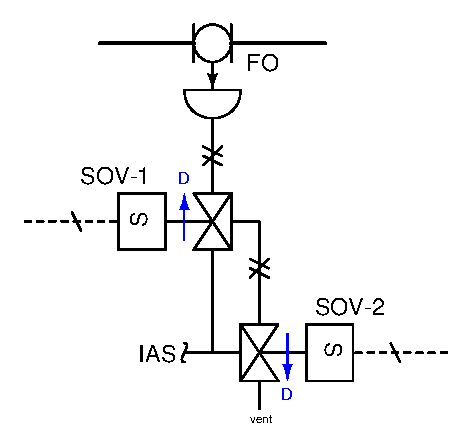
\includegraphics[width=15.5cm]{i01367x01.eps}$$

% Ingen blanklinjer er tillatt mellom linjer i en \halign-struktur!
% Jeg bruker kommentarer (%) i stedet, slik at TeX ikke feiler.

$$\vbox{\offinterlineskip
\halign{\strut
\vrule \quad\hfil # \ \hfil & 
\vrule \quad\hfil # \ \hfil & 
\vrule \quad\hfil # \ \hfil & 
\vrule \quad\hfil # \ \hfil \vrule \cr
\noalign{\hrule}
%
% Første rad
{\bf SOV-1 tilstand} & {\bf SOV-2 tilstand} & {\bf Åpen} & {\bf Stengt} \cr
%
\noalign{\hrule}
%
% Neste rad
De-energisert & De-energisert &  &  \cr
%
\noalign{\hrule}
%
% Neste rad
De-energisert & Energisert &  &  \cr
%
\noalign{\hrule}
%
% Neste rad
Energisert & De-energisert &  &  \cr
%
\noalign{\hrule}
%
% Neste rad
Energisert & Energisert &  &  \cr
%
\noalign{\hrule}
} % Slutt på \halign
}$$ % Slutt på \vbox

\underbar{file i01367}
%(END_QUESTION)





%(BEGIN_ANSWER)

% Ingen blanklinjer er tillatt mellom linjer i en \halign-struktur!
% Jeg bruker kommentarer (%) i stedet, slik at TeX ikke feiler.

$$\vbox{\offinterlineskip
\halign{\strut
\vrule \quad\hfil # \ \hfil & 
\vrule \quad\hfil # \ \hfil & 
\vrule \quad\hfil # \ \hfil & 
\vrule \quad\hfil # \ \hfil \vrule \cr
\noalign{\hrule}
%
% Første rad
{\bf SOV-1 tilstand} & {\bf SOV-2 tilstand} & {\bf Åpen} & {\bf Stengt} \cr
%
\noalign{\hrule}
%
% Neste rad
De-energisert & De-energisert &  & $\surd$ \cr
%
\noalign{\hrule}
%
% Neste rad
De-energisert & Energisert &  & $\surd$ \cr
%
\noalign{\hrule}
%
% Neste rad
Energisert & De-energisert & $\surd$ &  \cr
%
\noalign{\hrule}
%
% Neste rad
Energisert & Energisert &  & $\surd$ \cr
%
\noalign{\hrule}
} % Slutt på \halign
}$$ % Slutt på \vbox

%(END_ANSWER)





%(BEGIN_NOTES)

{\bf Dette spørsmålet er ment kun for eksamener, ikke for arbeidsark!}.

%(END_NOTES)

